% Chapter 5: Results and Discussion
This chapter presents the experimental results, comparing model performances across head, middle, and tail classes, and discusses the impact of different model architectures combined with different loss functions. First, the main findings are presented, followed by a detailed analysis of the results across experiments, and lastly a discussion of the results. 

\section{Main Findings}
Across all models, Balanced Softmax Loss demonstrated the highest performance on tail classes for models trained on long-tailed datasets while maintaining consistent performance on head, middle, and overall long-tailed test sets. The highest top-1 accuracy for tail classes was achieved by the ResNet50 architecture (Acc1: 0.6053), closely followed by the ConvNeXt Base architecture (Acc1: 0.5789). However, this improved tail-class performance comes at the cost of head-class accuracy, where ConvNeXt Base outperforms ResNet50 with a top-1 accuracy of 0.8685 compared to 0.8270. Overall, ConvNeXt Base demonstrates better performance across all classes (Acc1: 0.8230) compared to ResNet50 (Acc1: 0.7916). See Tables \ref{tab:resnet_lt_acc1_1} and \ref{tab:conv_lt_acc1_1} for reference. These findings, however, require further statistical analysis to confirm their significance and that the observed differences are not simply due to random variability.

Class-Balanced Loss consistently underperformed, warranting further investigation into its implementation. Similarly, the ViT-B/16 architecture demonstrated the lowest overall accuracy when trained on both balanced and long-tailed datasets (Acc1: 59.06 \%, see Table \ref{tab:vit_bal_acc1_1}), despite having the highest reported benchmark performance (Acc1: 93.95 \%) among all model architectures investigated in this thesis \cite{Tseng_2022}. This discrepancy suggests that the ViT-B/16 configuration used for the experiments in this thesis may not be well-suited for smaller-scale datasets such as CIFAR-100 without additional optimization steps. As discussed in sections \ref{sec:ViTs} and \ref{sec:model_selection}, changes in parameters may be required to reach its reported benchmarks. 

\section{Overall Results}
This section presents the overall results of all experiments conducted in this thesis, commenting on the best and worst performance of each loss design on a given model, and not directly comparing loss designs or models. It provides an overview of all findings to understand how each combination of architecture and loss function behaves.

\subsection{MobileNetV2}

\subsubsection{Results from Balanced Training}

\begin{table}[H]
    \centering
    \caption{Top-1 accuracy results for MobileNetV2 on the balanced dataset across all loss functions.}
    \begin{tabular}{cccccc}
        \toprule
        Loss Function & Balanced & Long-tailed & Head & Middle & Tail \\ 
        \midrule
        Softmax   & 0.7978   & \textbf{0.8059} & \textbf{0.8069} & \textbf{0.7870} & 0.8684 \\
        Focal loss   & 0.8014   & 0.8011 & 0.7998 & \textbf{0.7870} & 0.8947 \\
        Weighted Softmax loss   & 0.7978   & \textbf{0.8059} & \textbf{0.8069} & \textbf{0.7870} & 0.8684 \\
        Class-balanced loss   & 0.7978   & \textbf{0.8059} & \textbf{0.8069} & \textbf{0.7870} & 0.8684 \\
        Balanced Softmax loss   & \textbf{0.8034}  & 0.8030 & \textbf{0.8069} & 0.7574 & \textbf{0.9211} \\
        Equalization loss   & 0.7994   & 0.8040 & 0.8057 & 0.7692 & \textbf{0.9211} \\
        LDAM loss   &  0.7828   & 0.7821 & 0.7808 & 0.7574 & \textbf{0.9211} \\
        \bottomrule
    \end{tabular}
    \label{tab:mobilenet_bal_acc1_1}
\end{table}

% \begin{figure}[h!]
%     \centering
%     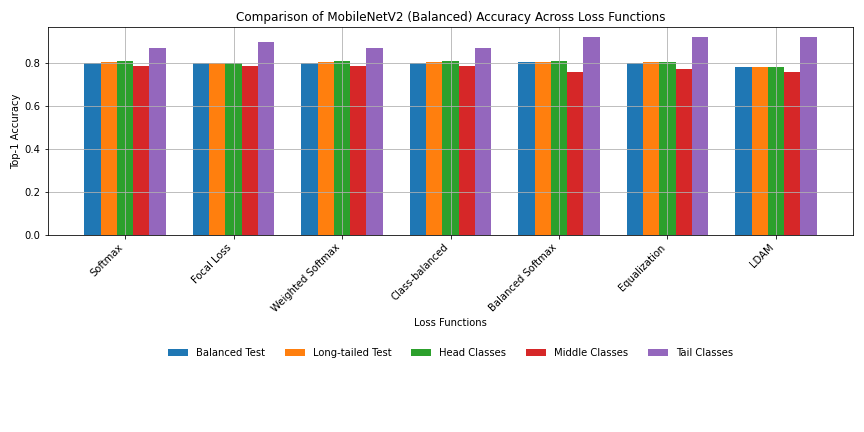
\includegraphics[width=\textwidth]{Images/Plots/mobilenet_bal_loss_comparison.png}
%     \caption{Top-1 accuracy comparison of MobileNetV2 trained on the balanced CIFAR-100 across loss functions on different test datasets. The bars represent performance on balanced test data, long-tailed test data, and head, middle, and tail classes.}
%     \label{fig:mobilenet_bal_loss_comparison}
% \end{figure}

From Table \ref{tab:mobilenet_bal_acc1_1}, Balanced Softmax Loss achieves the best accuracy on the balanced test dataset (Acc1: 0.8034) and the highest accuracy on tail classes (Acc1: 0.9211). Softmax, Weighted Softmax, and Class-Balanced Loss yield the same accuracies across all test datasets, likely due to shared cross-entropy-based designs that become indistinguishable when trained on balanced data \todo{reference to background section}. Although LDAM Loss demonstrates lower overall accuracy, its high tail-class accuracy matches that of Balanced Softmax and Equalization Loss, suggesting that tail-class performance may have reached a saturation point due to the limited number of samples in tail classes. This notion is further supported by differences in middle-class accuracy and identical performance across multiple long-tailed subsets, suggesting potential limitations in class-specific data quality or quantity.

\todo{Possibly add something about conducting the same experiments with a larger dataset to asses the observed saturation trend.}

\todo{Mention the overall performance of the six long-tail loss compared to the softmax baseline.}

\todo{Compare with table \ref{tab:benchmark_comparison}.}

\subsubsection{Results from Long-Tailed Training}

\begin{table}[H]
    \centering
    \caption{Top-1 accuracy results for MobileNetV2 on the long-tailed dataset across all loss functions.}
    \begin{tabular}{cccccc}
        \toprule
        Loss Function & Balanced & Long-tailed & Head & Middle & Tail \\ 
        \midrule
        Softmax   & 0.5282   & 0.7735 & 0.8341 & 0.5917 & 0.2368 \\
        Focal loss   & 0.5200   & \textbf{0.7745} & \textbf{0.8389} & 0.5917 & 0.1579 \\
        Weighted Softmax loss   & 0.5016   & 0.7231 & 0.7808 & 0.5503 & 0.2105 \\
        Class-balanced loss   & 0.1936   & 0.0913 & 0.0521 & 0.2485 & 0.2632 \\
        Balanced Softmax loss   & \textbf{0.5796}   & 0.7650 & 0.8069 & \textbf{0.6331} & \textbf{0.4211} \\
        Equalization loss   & 0.5310   & 0.7650 & 0.8235 & 0.5917 & 0.2368 \\
        LDAM loss   & 0.4264 & 0.5899 & 0.6137 & 0.5444 & 0.2632 \\
        \bottomrule
    \end{tabular}
    \label{tab:mobilenet_lt_acc1_1}
\end{table}

% \begin{figure}[h!]
%     \centering
%     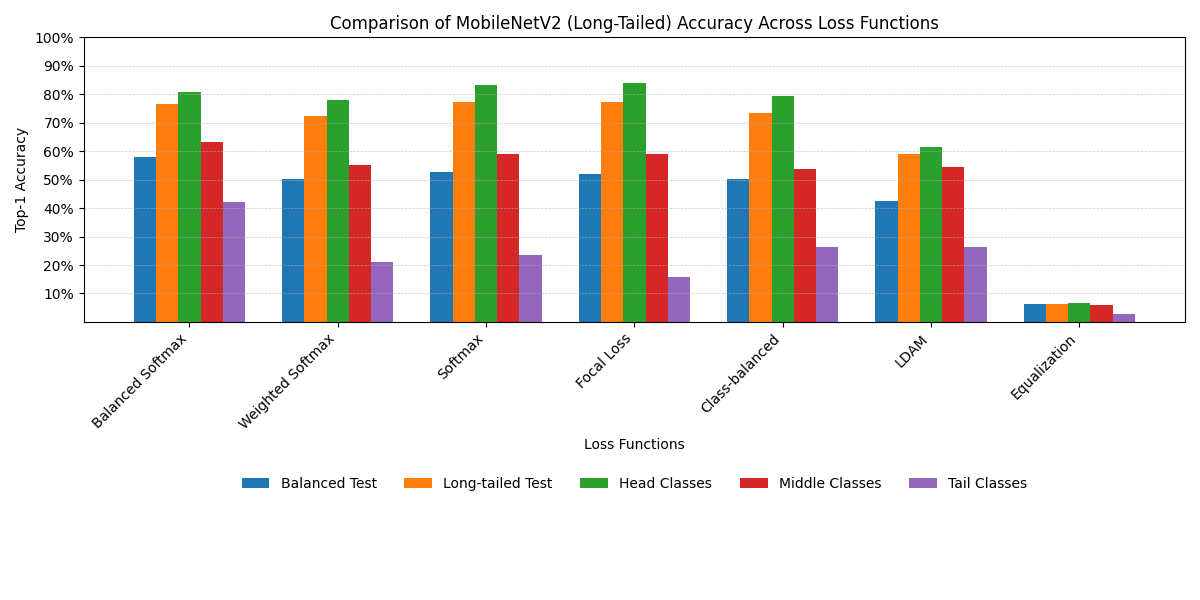
\includegraphics[width=\textwidth]{Images/Plots/mobilenet_lt_loss_comparison.png}
%     \caption{Top-1 accuracy comparison of MobileNetV2 trained on the long-tailed CIFAR-100 across loss functions on different test datasets. The bars represent performance on balanced test data, long-tailed test data, and head, middle, and tail classes.}
%     \label{fig:mobilenet_lt_loss_comparison}
% \end{figure}

FFrom Table \ref{tab:resnet_lt_acc1_1}, Balanced Softmax Loss significantly improves tail-class accuracy (0.6053), outperforming other losses, which also true for balanced and middle sets. Focal Loss achieves the best performance on the long-tailed dataset and head classes, indicating that while Balanced Softmax improves minority-class accuracy, Focal Loss remains strong for majority classes. Class-Balanced Loss and LDAM Loss both show underwhelming results, pointing toward the necessity of further tuning or combined methods (e.g., LDAM with DRW).

% Unlike the performance of loss functions trained on the balanced CIFAR100, there are not as many incidents of accuracies of the same value, except for the performance of Softmax Loss, Focal Loss, and Equalization loss on middle classes (Acc1: 0.5917). However, this value is not the highest, as the Balanced Softmax Loss achieves a top-1 accuracy of 0.6331. \todo{explain this.}

\todo{Compare with softmax baseline.}

\subsection{ResNet50}

\subsubsection{Results from Balanced Training}

\begin{table}[H]
    \centering
    \caption{Evaluation results for ResNet50 trained on the custom balanced dataset, showing Acc1.}
    \begin{tabular}{cccccc}
        \toprule
        Loss Function & Balanced & Long-tailed & Head & Middle & Tail \\ 
        \midrule
        Softmax loss   & \textbf{0.8324}  & 0.8421 & 0.8448 & 0.8047 & \textbf{0.9474} \\
        Focal loss   & 0.8310  & 0.8344 & 0.8341 & \textbf{0.8166} & 0.9211 \\
        Weighted Softmax loss   & \textbf{0.8324} & 0.8421 & 0.8448 & 0.8047 & \textbf{0.9474} \\
        Class-balanced loss   &  \textbf{0.8324} & 0.8421 & 0.8448 & 0.8047 & \textbf{0.9474} \\
        Balanced Softmax loss   & 0.8310 & \textbf{0.8430} & \textbf{0.8460} & 0.8107 & 0.9211 \\
        Equalization loss   & 0.8292 & 0.8373 & 0.8412 & 0.7929 & \textbf{0.9474} \\
        LDAM loss   & 0.7990 & 0.7983 & 0.8069 & 0.7337 & 0.8947 \\
        \bottomrule
    \end{tabular}
    \label{tab:resnet_bal_acc1_1}
\end{table}

From Table \ref{tab:resnet_bal_acc1_1}, Softmax, Weighted Softmax, and Class-Balanced Loss yield identical performance when trained on balanced data due to their cross-entropy-based base \todo{reference to background section}. Balanced Softmax Loss, by contrast, demonstrates strong performance on the long-tailed test set (0.8430) and head classes (0.8460), while still performing comparably on tail classes. LDAM Loss trails behind, suggesting that without additional adjustments such as deferred re-weighting (DRW) \cite{cao2019learningimbalanceddatasetslabeldistributionaware}, LDAM may not fully leverage its margin-based design.

\todo{compare to softmax baseline.}

\subsubsection{Results from Long-Tailed Training}

\begin{table}[H]
    \centering
    \caption{Evaluation results for ResNet50 trained on the long-tailed dataset, showing Acc1.}
    \begin{tabular}{cccccc}
        \toprule
        Loss Function & Balanced & Long-tailed & Head & Middle & Tail \\ 
        \midrule
        Softmax loss   & 0.5522 & \textbf{0.7954} & \textbf{0.8531} & 0.6391 & 0.2105 \\
        Focal loss   & 0.5456 & 0.7935 & 0.8483 & 0.6272 & 0.3158 \\
        Weighted Softmax loss   & 0.4976 & 0.7336 & 0.7915 & 0.5562 & 0.2368 \\
        Class-balanced loss   & 0.2052 & 0.1836 &  0.1445 & 0.3787 & 0.1842 \\
        Balanced Softmax loss   & \textbf{0.5908} & 0.7916 & 0.8270 & \textbf{0.6568} & \textbf{0.6053} \\
        Equalization loss   & 0.5452 & 0.7897 & 0.8389 & 0.6450 & 0.3421 \\
        LDAM loss   & 0.3742 & 0.5937 & 0.6469 & 0.4438 & 0.0789 \\
        \bottomrule
    \end{tabular}
    \label{tab:resnet_lt_acc1_1}
\end{table}

From Table \ref{tab:resnet_lt_acc1_1}, Balanced Softmax Loss significantly improves tail-class accuracy (0.6053), outperforming other losses, while also outperforming on balanced and middle sets. Softmax Loss achieves the best performance on the long-tailed dataset and head classes, indicating that while Balanced Softmax improves minority-class accuracy, Softmax remains strong for majority classes. Class-Balanced Loss and LDAM Loss both show underwhelming results, pointing toward the necessity of further tuning or combined methods (e.g., LDAM with DRW). 

\subsection{ViT-B/16}

\subsubsection{Results from Balanced Training}

\begin{table}[H]
    \centering
    \caption{Evaluation results for ViT-B/16 trained on the custom balanced dataset, showing Acc1.}
    \begin{tabular}{cccccc}
        \toprule
        Loss Function & Balanced & Long-tailed & Head & Middle & Tail \\ 
        \midrule
        Softmax loss   & 0.5620 & 0.5671 & 0.5521 & 0.6036 & 0.7368 \\
        Focal loss   & 0.5516 & 0.5538 & 0.5438 & 0.5680 & 0.7105 \\
        Weighted Softmax loss   & 0.5620 & 0.5671 & 0.5521 & 0.6036 & 0.7368 \\
        Class-balanced loss   & 0.5620 & 0.5671 &  0.5521 & 0.6036 & 0.7368 \\
        Balanced Softmax loss   & 0.5628 & 0.5642 & 0.5640 & 0.5325 & 0.7105 \\
        Equalization loss   & 0.5634   & 0.5519 & 0.5462 & 0.5503 & 0.6842 \\
        LDAM loss   & \textbf{0.5906} &  \textbf{0.6013} & \textbf{0.5924} & \textbf{0.6095} & \textbf{0.7632} \\
        \bottomrule
    \end{tabular}
    \label{tab:vit_bal_acc1_1}
\end{table}

From Table \ref{tab:vit_bal_acc1_1}, LDAM Loss achieves the overall best performance for ViT-B/16 trained on balanced data. However, the overall performance remain far below the benchmark results for Vision Transformers on CIFAR-100, see table \ref{tab:benchmark_comparison}. This suggests that further adjustments are needed, possibly including extended training time, data augmentation, or different optimizers, see \ref{sec:ViTs}. 

\subsubsection{Results from Long-Tailed Training}

\begin{table}[h!]
    \centering
    \caption{Evaluation results for ViT-B/16 trained on the long-tailed dataset, showing Acc1.}
    \begin{tabular}{cccccc}
        \toprule
        Loss Function & Balanced & Long-tailed & Head & Middle & Tail \\ 
        \midrule
        Softmax loss   & 0.2254 & \textbf{0.4367} & \textbf{0.5071} & 0.1775 & 0.0263 \\
        Focal loss   & 0.2210 & 0.4206 & 0.4834 & 0.1953 & 0.0263 \\
        Weighted Softmax loss   & 0.1284 & 0.1760 & 0.1919 & 0.1302 & 0.0263 \\
        Class-balanced loss   & 0.0558 & 0.0076 & 0.0000 & 0.0237 & \textbf{0.1053} \\
        Balanced Softmax loss   & \textbf{0.2460} & 0.4244 & 0.4822 &  \textbf{0.2130} & 0.0789 \\
        Equalization loss   & 0.2168 & 0.4215 & 0.4893 & 0.1716 & 0.0263 \\
        LDAM loss   & 0.1570 & 0.2750 & 0.3140 & 0.1361 & 0.0263 \\
        \bottomrule
    \end{tabular}
    \label{tab:vit_lt_acc1}
\end{table}

From Table \ref{tab:vit_lt_acc1}, performance remains low across all loss functions. Balanced Softmax Loss slightly improves results on balanced and middle categories, while Softmax Loss achieves the highest accuracy on the long-tailed dataset and head classes. However, these gains are modest. The best accuracy on tail classes (0.1053) is achieved by Class-Balanced Loss, though it fails everywhere else. This pattern suggests that the ViT-B/16 architecture may not be sufficient for robust performance on smaller-scale, long-tailed datasets and may require major adjustments or pre-training on larger datasets, see section \ref{sec:ViTs}. The results underscore the challenges in directly applying transformer-based models to imbalanced scenarios without significant considerations.

\subsection{ConvNeXt Base}

\subsubsection{Results from balanced Training Dataset}

\begin{table}[h!]
    \centering
    \caption{Evaluation results for ConvNeXt Base trained on the custom balanced dataset, showing Acc1.}
    \begin{tabular}{cccccc}
        \toprule
        Loss Function & Balanced & Long-tailed & Head & Middle & Tail \\ 
        \midrule
        Softmax loss   & 0.8332 & \textbf{0.8535} & \textbf{0.8566} & 0.8166 & \textbf{0.9474} \\
        Focal loss   & 0.8314 & 0.8487 & 0.8507 & 0.8284 & 0.8947 \\
        Weighted Softmax loss   & 0.8332 & \textbf{0.8535} & \textbf{0.8566} &  0.8166 & \textbf{0.9474} \\
        Class-balanced loss   & 0.8332 & \textbf{0.8535} & \textbf{0.8566} & 0.8166 & \textbf{0.9474} \\
        Balanced Softmax loss   & \textbf{0.8364} & 0.8344 & 0.8365 & 0.7988 & \textbf{0.9474} \\
        Equalization loss   & 0.8318 & 0.8468 & 0.8448 & \textbf{0.8343} & \textbf{0.9474} \\
        LDAM loss   & 0.8316 & 0.8373 & 0.8412 & 0.8047 & 0.8947 \\
        \bottomrule
    \end{tabular}
    \label{tab:conv_bal_acc1_1}
\end{table}

From table \ref{tab:conv_bal_acc1_1}, the best performance on the balanced test dataset is achieved by the Balanced Softmax Loss (Acc1: 0.8364), while also achieving the best result on the tail classes (Acc1: 0.9474).

Not surprisingly, the Softmax loss, Weighted Softmax loss, and Class-balanced loss exhibits the same performance across all test dataset, as they were trained with the balanced training dataset, and their designs reduces to the Softmax loss. These three loss function exhibit the best performance on the long-tailed dataset (0.8535), head classes (Acc1: 0.8566) and tail classes (Acc1: 0.9474). The best performance on middle classes is achieved my the Equalization loss (Acc1: 0.8343).

Five out of six loss design achieve the same performance on the tail classes, likely due to saturation causes by the limited number of samples and noise.

\todo{Explain why balanced softmax could achieve higher accuracy in the balanced dataset.}

\subsubsection{Results from Long-Tailed Training Dataset}


\begin{table}[h!]
    \centering
    \caption{Evaluation results for ConvNeXt Basetrained on the long-tailed dataset, showing Acc1.}
    \begin{tabular}{cccccc}
        \toprule
        Loss Function & Balanced & Long-tailed & Head & Middle & Tail \\ 
        \midrule
        Softmax loss   & 0.5972 & \textbf{0.8316} & \textbf{0.8898} & 0.6568 & 0.3158 \\
        Focal loss   & 0.5938 & 0.8145 & 0.8685 & 0.6568 & 0.3158 \\
        Weighted Softmax loss   & 0.4090 & 0.6356 & 0.6848 & 0.4911 & 0.1842 \\
        Class-balanced loss   & 0.0142 & 0.0019 & 0.0000 & 0.0000 & 0.0526 \\
        Balanced Softmax loss   & \textbf{0.6460} & 0.8230 & 0.8685 & 0.6509 & \textbf{0.5789} \\
        Equalization loss   & 0.5956 & 0.8278 & 0.8768 & \textbf{0.6923} & 0.3421 \\
        LDAM loss   & 0.3770 & 0.5956 & 0.6445 & 0.4260 & 0.2632 \\
        \bottomrule
    \end{tabular}
    \label{tab:conv_lt_acc1_1}
\end{table}

From table \ref{tab:conv_lt_acc1_1} the best performance on a balanced test dataset is achived by the Balanced Softmax loss (Acc1: 0.6460), which was the same for the ConvNeXt Base trained with the balanced CIFAR100. See table \ref{tab:conv_bal_acc1_1}. Likewise, the Balanced Softmax loss performs with the highest accuracy on the tail classes (Acc1: 0.5789), far exceeding the second highest performance, achieved by Equalization loss (Acc1: 0.3421). The highest accuracy on the long-tailed dataset (Acc1: 0.8316), as well as the head classes (Acc1: 0.8898), is achieved by the Softmax Loss, while Equalization Loss performs with highest accuracy on middle classes (Acc1: 0.6923). In comparison, the Balanced Softmax loss is third in accuracy on the long-tailed dataset, head classes, as well as middle classes. 

Noticably, both Softmax loss and focal loss performs with equal accuracies on both middle (Acc1: 0.6568) and tail classes (Acc1: 0.3158), but not elsewhere. \todo{give a reason why that might be.}

The worst performance is achieved by the Class-Balanced loss, with accuracies far below the second worst performances. The Class-balanced loss should be disregarded for training with a long-tailed dataset, as it is most likely a fault in implementation. \todo{investigate this and return to this conclusion.}

\section{Comparison with Benchmarks}
Table \ref{tab:benchmark_comparison} compares the best results from the models trained on the balanced CIFAR-100 dataset in this thesis with published benchmarks using the same or similar architectures. This comparison serves as a reference to ensure the results align with expectations and to identify any potential discrepancies. 

\begin{table}[H]
    \centering
    \caption{Comparison of model performance on balanced CIFAR-100 with published benchmarks.}
    \begin{tabular}{|l|c|c|}
    \hline
    \textbf{Model}        & \textbf{Result (Acc1)} & \textbf{Benchmark Result (Acc1)}  \\ \hline
    MobileNetV2           & 80.34\%               & 73.20\% \cite{park2022bitatneuralnetworkbinarization}  \\ \hline
    ResNet50            & 83.24\%               & 86.90\% \cite{wightman2021resnetstrikesbackimproved}  \\ \hline
    ViT-B/16              & 59.06\%               & 93.95\% \cite{Tseng_2022} \\ \hline
    ConvNeXt Base         & 83.64\%               & 83.82\% \cite{10072172}  \\ \hline
    \end{tabular}
    \label{tab:benchmark_comparison}
\end{table}

Notably, there are no published benchmarks for ConvNeXt Base trained on CIFAR-100. The closest benchmark available is from Feng et al. \cite{10072172}, where Conv2NeXt achieved a top-1 accuracy of 83.82\%, which is highly similar to the result obtained here.

For MobileNetV2, the results in this thesis surpass the published benchmarks. This could be attributed to improved loss function designs. On the other hand, ResNet50 exhibits a slightly lower accuracy compared to benchmarks, which may be explained by differences in optimization strategies, such as the use of Adam optimizer instead of SGD \cite{menon2021longtaillearninglogitadjustment}.

The most significant deviation is observed with ViT-B/16, where the accuracy falls far short of the benchmark. This discrepancy suggests that the configuration for ViT-B/16 may not be well-suited for the smaller-scale CIFAR-100 dataset. 

Overall, these results indicate that the experimental setup is effective for most models but highlights potential limitations for transformer-based architectures such as ViT-B/16. Future investigation is necessary to understand and address these discrepancies.


\section{Comparison of Models}

The model are compared by taking the mean of the results of the loss functions for each model. The mean and standard deviation for each model are shown on figure \ref{fig:mean_loss_comparison_line}, and on figure \ref{fig:mean_loss_comparison_line_noCB} excluding the Class-Balanced Loss.


\begin{figure}[h!]
    \centering
    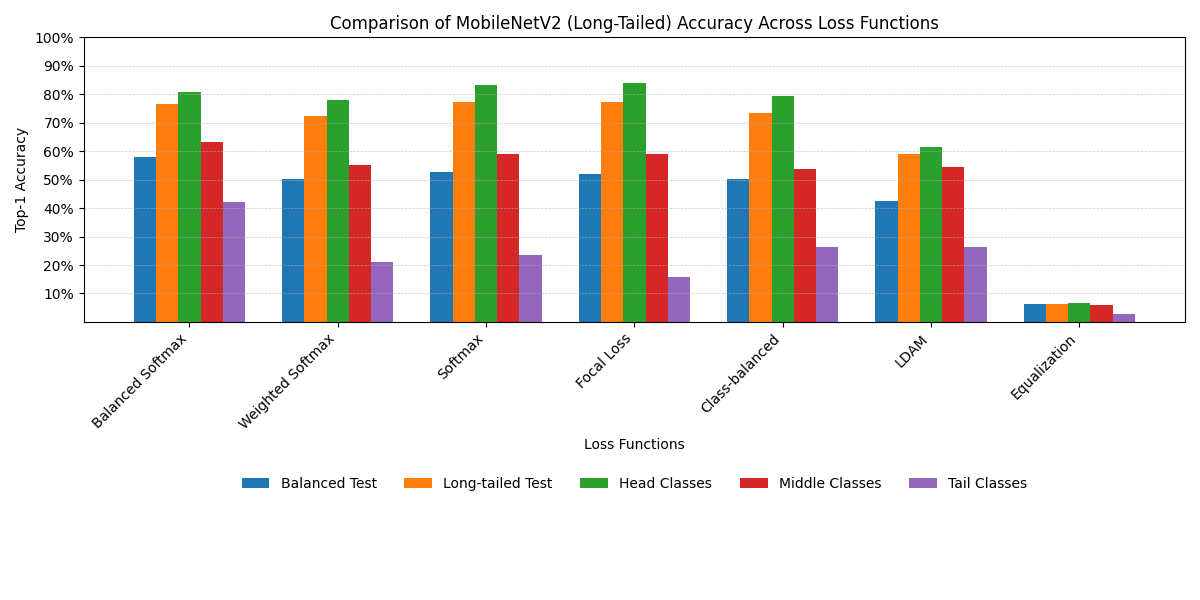
\includegraphics[width=\textwidth]{Images/Plots/mobilenet_lt_loss_comparison.png}
    \caption{MobileNetV2 top 1 accuracy across test categories (Balanced, Long-tailed, Head, Middle, Tail) for different loss functions.}
    \label{fig:mobilenet_lt_loss_comparison}
\end{figure}

\begin{figure}[h!]
    \centering
    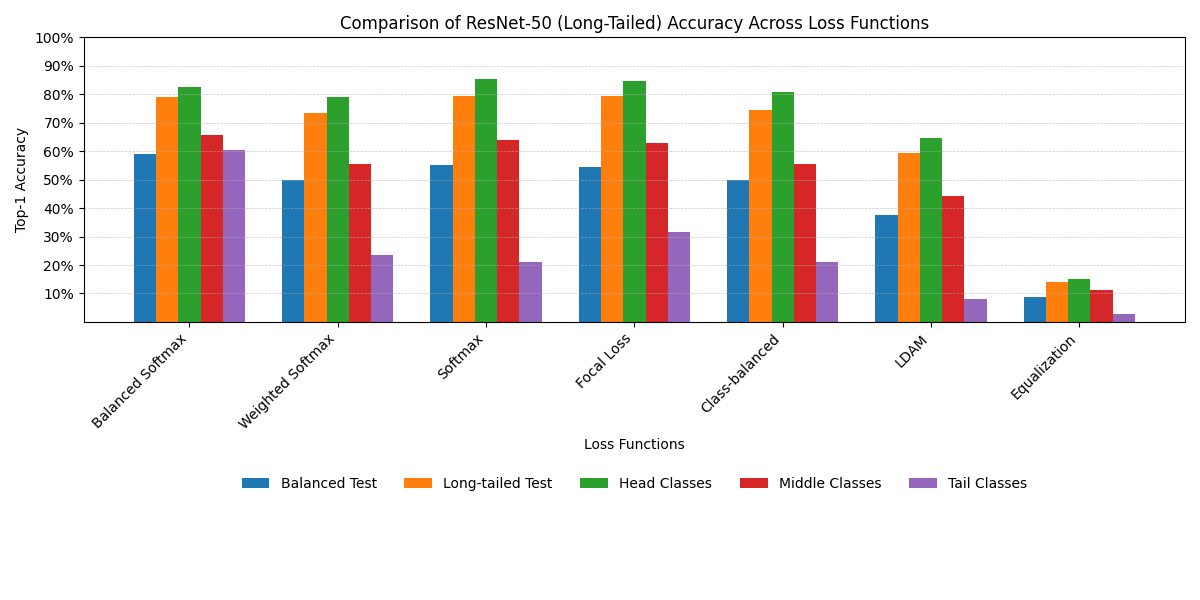
\includegraphics[width=\textwidth]{Images/Plots/resnet_lt_loss_comparison.png}
    \caption{ResNet50 top 1 accuracy across test categories (Balanced, Long-tailed, Head, Middle, Tail) for different loss functions.}
    \label{fig:resnet_lt_loss_comparison}
\end{figure}

\begin{figure}[h!]
    \centering
    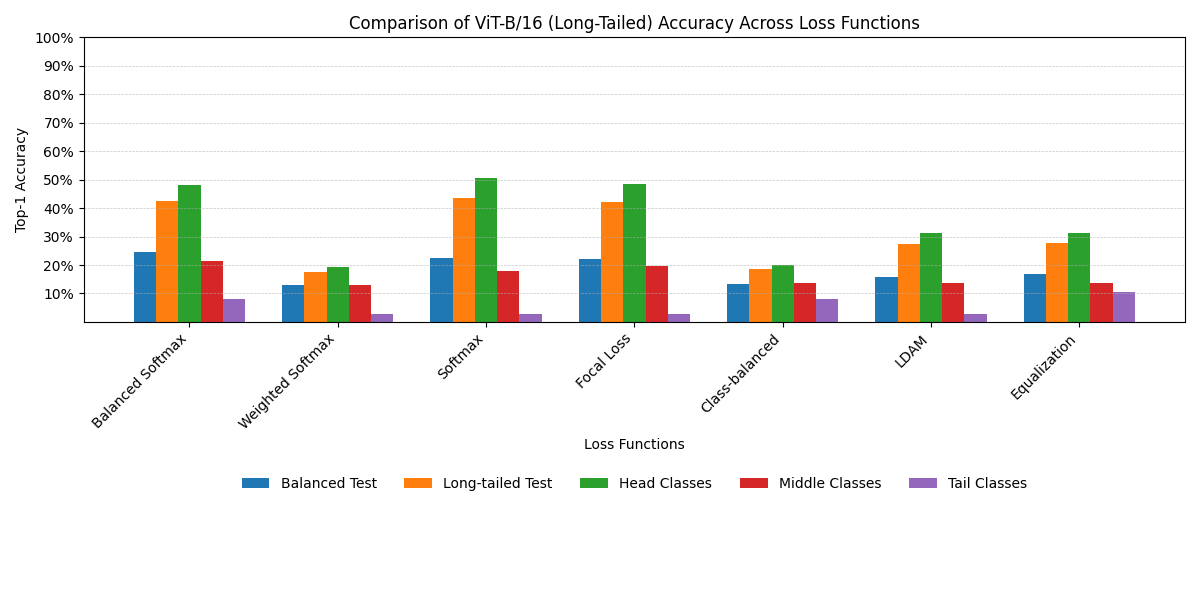
\includegraphics[width=\textwidth]{Images/Plots/vit_lt_loss_comparison.png}
    \caption{ViT-B/16 top 1 accuracy across test categories (Balanced, Long-tailed, Head, Middle, Tail) for different loss functions.}
    \label{fig:vit_lt_loss_comparison}
\end{figure}

\begin{figure}[h!]
    \centering
    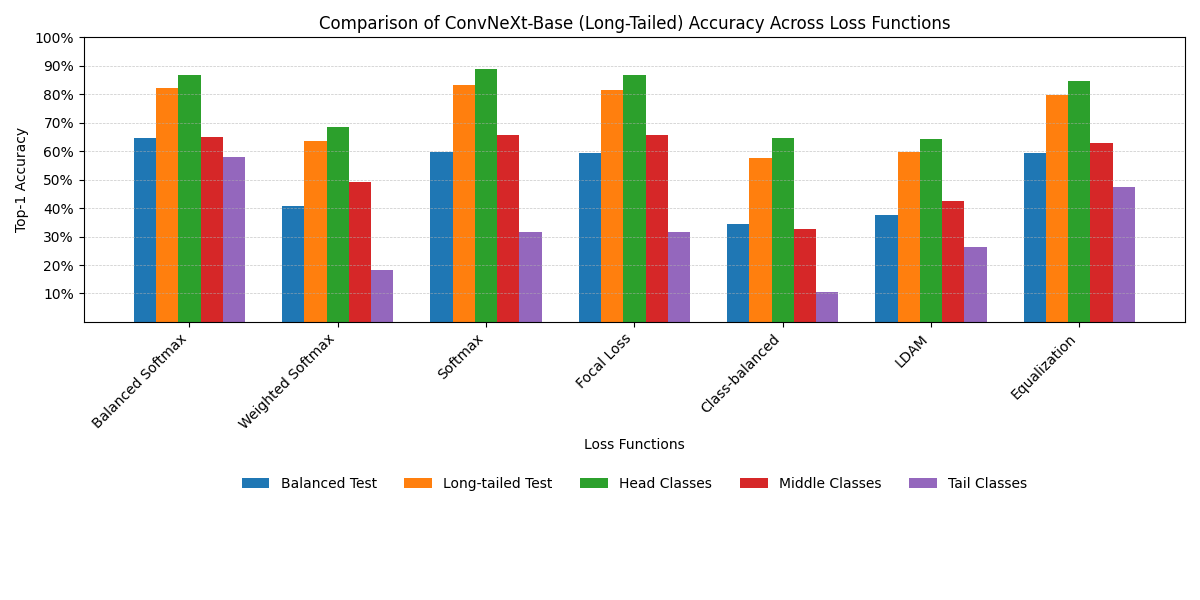
\includegraphics[width=\textwidth]{Images/Plots/convnext_lt_loss_comparison.png}
    \caption{ConvNeXt Base top 1 accuracy across test categories (Balanced, Long-tailed, Head, Middle, Tail) for different loss functions.}
    \label{fig:conv_lt_loss_comparison}
\end{figure}

\subsubsection{Mean and Standard Deviation}


The plots on figures \ref{fig:mean_loss_comparison_line} and \ref{fig:mean_loss_comparison_line_noCB} compares the performance of the models MobileNetV2, ResNet50, ViT-B/16, and ConvNeXt Base across the evaluation categories: balanced, long-tailed, head, middle, and tail. Each model is slightly offset along the x-axis to avoid overlap. The mean and standard deviation in figure \ref{fig:mean_loss_comparison_line} include the Class-Balanced Loss while figure \ref{fig:mean_loss_comparison_line_noCB} does not.

Each point represents the mean accuracy of a model for a specific category and the bars represent the standard deviation. A model with higher mean accuracy is performing better in that category, and a smoother or higher line indicates consistent performance across all categories.

The error bars show the variability in accuracy across different loss functions for each model and category. A longer error bar means the performance is less consistent and the performance is more dependent on the chosen loss function, while shorter error bars indicate consistant performance.

The plot in figure \ref{fig:mean_loss_comparison_line_noCB} shows that the model with the best average performance on tail classes is the ConvNeXt Base architecture, while also showing a strong performance in other categories. 

MobileNetV2 is the least dependent on loss functions, exhibiting the smallest standard deviation, while the ResNet50 architecture, compared with figures \ref{fig:resnet_bal_loss_comparison_line} and \ref{fig:conv_bal_loss_comparison_line}, is the most dependent on loss functions when exhibiting tail performance, as the Balanced Softmax Loss outperforms the remaining loss functions, as seen in figure \ref{fig:resnet_bal_loss_comparison_line} and table \ref{tab:resnet_lt_acc1_1}.

The model exhibiting the worst performance is the ViT-B/16 with a significant lower mean than the other three models. \todo{reference to figures and tables.}

% \begin{figure}[h!]
%     \centering
%     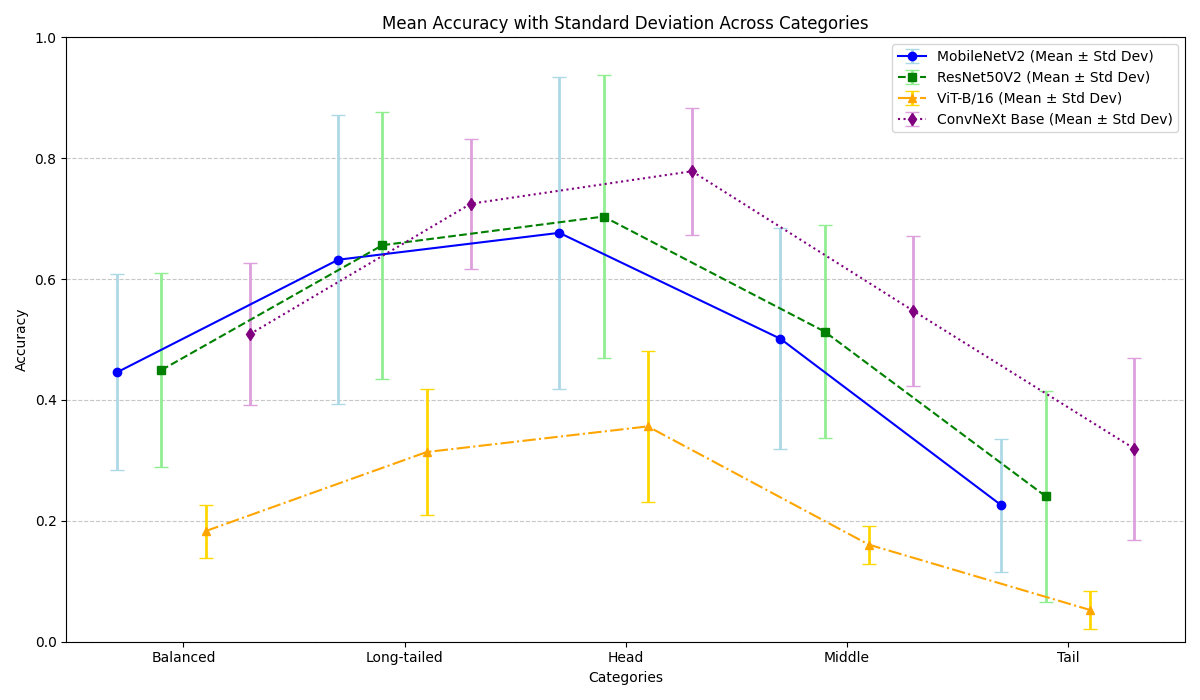
\includegraphics[width=\textwidth]{Images/Plots/mean_loss_comparison.png}
%     \caption{Mean Accuracy with Standard Deviation Across Categories for MobileNetV2, ResNet50, ViT-B/16, and ConvNeXt Base.}
%     \label{fig:mean_loss_comparison_line}
% \end{figure}

\begin{figure}[h!]
    \centering
    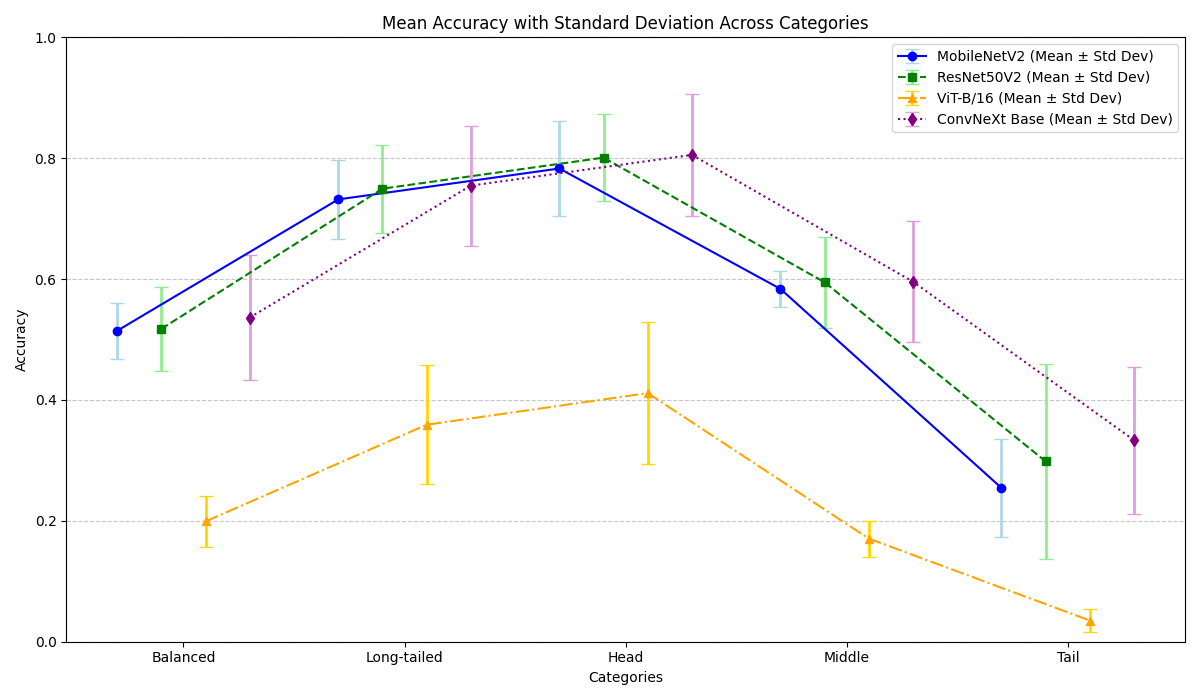
\includegraphics[width=\textwidth]{Images/Plots/mean_loss_comparison_noCB.png}
    \caption{Mean Accuracy with Standard Deviation Across Categories for MobileNetV2, ResNet50, ViT-B/16, and ConvNeXt Base without Class-Balanced Loss.}
    \label{fig:mean_loss_comparison_line_noCB}
\end{figure}


\todo{Comparison of overall model performance. Potentially statistical analysis, e.g. ANOVA, Tukey's HSD.}

\section{Comparison of Loss Functions}
\todo{Comment on the lack of results from the Class-Balanced Loss on all sets except the tail classes.} 

From figure \ref{fig:loss_comparison_bars} it can be seen that the Balanced Softmax Loss has a better average perfomance on tail classes, while also displaying the smoothest variation across evaluation categories, ignoring the Class-Balanced loss. However, the standard deviation suggests that the perfomance of the Balanced Softmax Loss depend on the model architecture.

% \begin{figure}[h!]
%     \centering
%     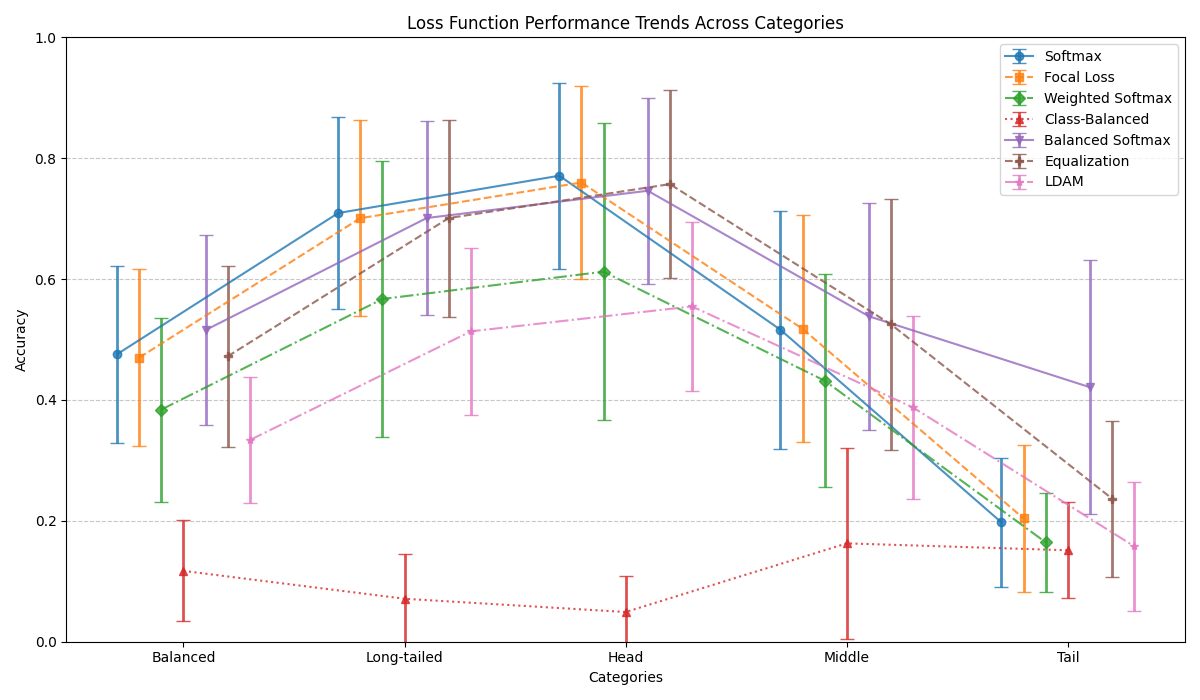
\includegraphics[width=\textwidth]{Images/Plots/loss_comparison.png}
%     \caption{Performance trends of different loss functions across evaluation categories. Error bars indicate the standard deviation of accuracy across models, highlighting variability in performance for each loss function.}
%     \label{fig:loss_comparison}
% \end{figure}


\begin{figure}[h!]
    \centering
    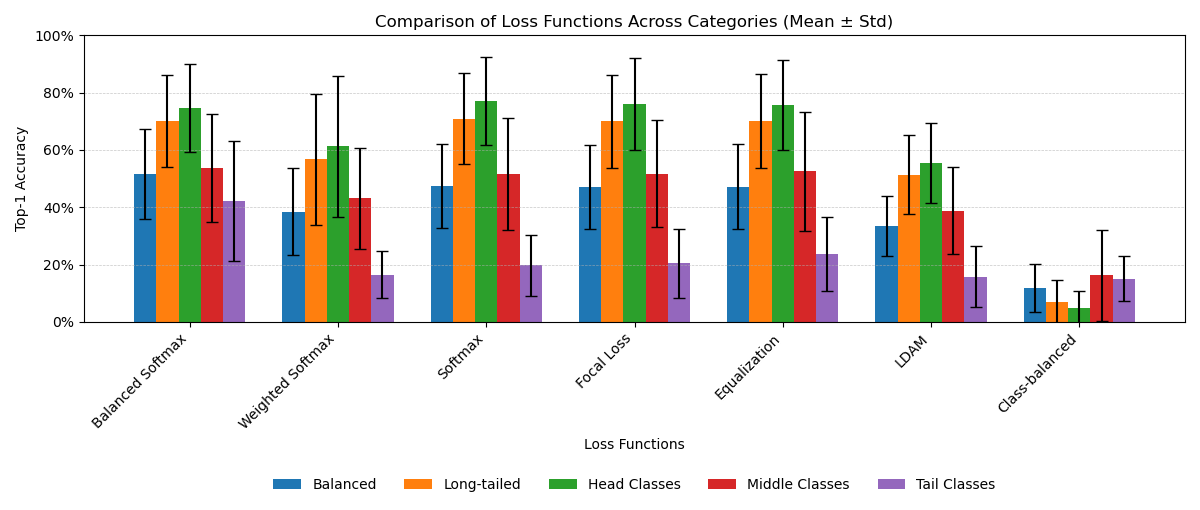
\includegraphics[width=\textwidth]{Images/Plots/loss_function_bar_plot_mean_std.png}
    \caption{Performance trends of different loss functions across evaluation categories. Error bars indicate the standard deviation of accuracy across models, highlighting variability in performance for each loss function.}
    \label{fig:loss_comparison_bars}
\end{figure}


\begin{table}[h!]
    \centering
    \caption{Performance Summary Across Categories (Mean ± Std)}
    \scriptsize
    \begin{tabular}{lccccc}
        \toprule
        Loss Function & Balanced & Long-tailed & Head & Middle & Tail \\
        \midrule
        Balanced Softmax & $0.5156 \pm 0.1577$ & $0.7010 \pm 0.1610$ & $0.7462 \pm 0.1540$ & $0.5385 \pm 0.1881$ & $0.4211 \pm 0.2097$ \\
        Weighted Softmax & $0.3841 \pm 0.1522$ & $0.5671 \pm 0.2290$ & $0.6123 \pm 0.2462$ & $0.4320 \pm 0.1761$ & $0.1645 \pm 0.0819$ \\
        Softmax & $0.4758 \pm 0.1466$ & $0.7093 \pm 0.1587$ & $0.7710 \pm 0.1537$ & $0.5163 \pm 0.1970$ & $0.1974 \pm 0.1061$ \\
        Focal Loss & $0.4701 \pm 0.1462$ & $0.7008 \pm 0.1624$ & $0.7598 \pm 0.1599$ & $0.5178 \pm 0.1876$ & $0.2039 \pm 0.1211$ \\
        Equalization & $0.4721 \pm 0.1494$ & $0.7010 \pm 0.1629$ & $0.7571 \pm 0.1558$ & $0.5252 \pm 0.2072$ & $0.2368 \pm 0.1289$ \\
        LDAM & $0.3504 \pm 0.1224$ & $0.5187 \pm 0.1443$ & $0.5548 \pm 0.1792$ & $0.3947 \pm 0.1886$ & $0.1587 \pm 0.1078$ \\
        Class-balanced & $0.1172 \pm 0.0814$ & $0.0711 \pm 0.0841$ & $0.0490 \pm 0.0624$ & $0.1628 \pm 0.1477$ & $0.1513 \pm 0.0946$ \\
        \bottomrule
    \end{tabular}
    \label{tab:performance_summary}
\end{table}
   

% \todo{Move benchmark results into a table.}

% Highlight Key Differences
% If there are differences in training conditions (e.g., data augmentation, optimization strategies, or hardware), acknowledge them:
% "It is important to note that while our setup involves an imbalanced CIFAR-100 dataset, the benchmark results were obtained on a balanced dataset."
% "Our experiments use an Adam optimizer, whereas [Source] employed SGD with momentum."

% \section{Qualitative Results}
% Include if time.
% Provide examples of correctly and incorrectly classified samples, especially for tail classes.
% Include visualizations or images of difficult cases to highlight challenges in tail-class prediction.

\section{Summary and Discussion}
Things for discussion:

\begin{itemize}
    \item Why is the performance on tail classes better than the performance on head and middle classes for the balanced training data, and what could it mean for the results on the long-tail training data?
    \item Running multiple of the same training to check for variance. What could this tell us in terms of statistical significance?
    \item The LDAM should be run with DRW as well. Compare to articles that run both LDAM and LDAM-DRW.
    \item Including or omitting the Class-Balanced Loss.
    \item Discuss why the ViT-B/16 model underperforms but shows excellent performance in other studies.
    \item Argue why the test data for CIFAR-100 was created from the training data instead of the validation data, and why or why not it would have been better to split the validation data instead.
\end{itemize}


The Balanced Softmax Loss proved to be the most effective loss function for tail classes, consistently achieving the highest accuracy on these classes across all models while also achieving competing results on other datasets. This results highlight its strenght in re-weighting logits to account for imbalanced datasets, particular for tail classes, where the Softmax baseline loss function falter. The synergy between Balanced Softmax and certain architectures, such as ConvNeXt Base, was espicially notable, suggesting that specific combinations of models and loss functions can achieve superior performance.

However, this improvement in tail-class accuracy often came with trade-offs. For example, while ResNet50 achieved a top 1 accuracy of 0.6053 on tail classes using Balanced Softmax, its head-class accuracy (0.8270) lagged behind ConvNeXt Base (0.8685). This trade-off highlights the challenge of optimizing for both head and tail classes simultaneously and indicates that Balanced Softmax prioritizes tail-class adjustments at the expense of head-class performance. \todo{mention statistical significance.}

Class-Balanced Loss, in contrast, consistently underperformed across all models and datasets. This discrepancy between its intended purpose and observed results suggests possible issues with its weighting strategy or implementation. Further investigation is necessary to understand these limitations and determine whether its performance can be improved.

Notably, the ViT-B/16 architecture underperformed significantly across all loss functions and datasets, with an the best accuracy of 59.06\% on a balanced training dataset compared to its benchmark of 93.95\%. This suggests that Vision Transformers, despite their reported success in other contexts, may require more data, longer training, or additional fine-tuning. The results indicate that the default ViT-B/16 architecture may not be well-suited for long-tailed datasets without further optimization.

While Balanced Softmax stood out as the most robust loss function overall, statistical validation is required to confirm the significance of these findings, particularly when comparing closely performing configurations. % For instance, the performance gap between Balanced Softmax and Softmax Loss on middle classes or long-tailed datasets could reflect inherent dataset characteristics rather than the superiority of the loss function alone.

Overall, these findings emphasize the importance of aligning loss functions with both dataset characteristics and model architectures to address the challenges of deep long-tailed learning. % They also highlight the need for a nuanced approach that balances improvements in tail-class accuracy with minimal trade-offs in head-class and overall performance.

\todo{Influence of optimizer} \url{https://arxiv.org/pdf/2007.07314v2} \url{https://openreview.net/pdf?id=rk6qdGgCZ}